\documentclass[preprint,12pt]{elsarticle}

\usepackage{lineno}
\usepackage{amsmath,amssymb}
\usepackage{booktabs}
\usepackage{longtable}
\usepackage{graphicx}
\usepackage{subcaption}
\usepackage{xcolor}
\usepackage{hyperref}
\hypersetup{colorlinks=true,linkcolor=blue,citecolor=blue,urlcolor=blue}

\journal{Neurocomputing}

% ---- convenience macros ----
\newcommand{\pp}{\,\mathrm{pp}}
\newcommand{\VERIFY}[1]{\textbf{\textcolor{red}{[VERIFY: #1]}}}

\begin{document}

\begin{frontmatter}

% TITLE PENDING AUTHOR DECISION (stage-8 pre-specified downgrade). Candidate T2:
% What Carries Deep-Noise Robustness in a Mamba-3 Block? Input-Independent Scans and Noise-Dependent Gating under Cross-Condition Shift
\title{Selectivity and Multiplicative Gating under Matched-Noise Cross-Condition Shift: Controlled Ablations of a Mamba-3 Block}

\author{Yi Wang\corref{cor1}}
\ead{jefflsxy@lsu.edu.cn}
\address{College of Engineering, Lishui University, Lishui 323000, Zhejiang, China}
\cortext[cor1]{Corresponding author}

\begin{abstract}
% DRAFT FOR AUTHOR APPROVAL (stage-8 pre-specified downgrade)
The robustness of Mamba-style selective state-space models is often attributed to input-dependent selectivity. We test this attribution with pre-specified ablations of one Mamba-3 block on bearing vibration data under cross-condition shift (XJTU-SY, one speed-and-load pair, training and evaluation bearings disjoint) with matched-noise training, reporting macro-F1 at the final epoch of a fixed budget. The central contrasts were re-run with training and evaluation noise drawn independently. Making the scan's dynamics and read/write coefficients input-independent ($\Delta$, $A$, $B$, $C$, trapezoidal weight and rotation angles) does not remove the block's advantage over a time-invariant S4D: the fully frozen block leads by $+21.3$, $+23.3$, $+20.3$\,pp at $0$, $-2$ and $-6$\,dB (all intervals excluding zero). Removing the multiplicative output gate costs $+9.4$, $+15.7$, $+27.0$\,pp in the partially frozen block and $+5.4$, $+9.3$, $+32.6$\,pp in the fully frozen block, resolved only at $-6$\,dB; without its gate the fully frozen block still exceeds S4D at $0$ and $-2$\,dB but falls below it at $-6$\,dB. Replacing the gate by an additive branch of identical size and initial weights leaves the result indistinguishable from removing it. Adding a gate to S4D recovers part of the gap, no more than an additive branch of the same size on one transition direction and slightly more on the other. On Paderborn data the gate-removal cost replicates when training and evaluation share bearings, the freeze advantage only at $-6$\,dB, and nothing replicates on disjoint bearings, where every architecture transfers poorly. The evidence supports input-independent scan coefficients sufficing in this block and a gate whose necessity grows with noise depth; it is limited to one block, one shift pair per dataset and five seeds.
\end{abstract}

\begin{keyword}
state-space models \sep Mamba \sep input selectivity \sep gating \sep robustness \sep ablation \sep distribution shift \sep matched-noise training
\end{keyword}

\end{frontmatter}

\linenumbers

\section{Introduction}
\label{sec:intro}

Selective state-space models (SSMs) of the Mamba family have rapidly become default sequence backbones, and a common narrative has formed around \emph{why} they work: input-dependent selectivity---the ability to modulate state dynamics per token---is credited with filtering noise, adapting to distribution shift, and outperforming time-invariant predecessors such as S4D~\cite{gu2023mamba}. \cite{qu2024mambasurvey,patro2024mamba360} This belief motivates a growing family of ``selective'' architectures, yet recent evidence questions it: a systematic comparison on 59 clean multivariate time-series classification benchmarks (MONSTER and UEA) finds the \emph{simpler, time-invariant} S4D consistently ahead of Mamba-family variants in accuracy and efficiency~\cite{saadatmand2026s4d}, and theoretical analyses identify expressivity regimes where Mamba is provably weaker~\cite{yu2025blockbiased}. Which account is right---and, more importantly, \emph{what exactly should be credited} when a Mamba-style block does prove robust? This paper addresses the second question for one block and one testbed, with a controlled ablation chain whose decision thresholds were fixed before each grid was run. The testbed is bearing vibration diagnosis under operating-condition drift and matched noise, in which the robustness gap is large (12--28$\pp$ between S4D and the frozen Mamba-3 blocks in the independent-noise results), the evaluation labels are identical across all cells of each transition (hash-verified), and the block can be dissected.

Failure to identify the source of an empirical gain is a recurring weakness of machine-learning scholarship~\cite{lipton2018troubling}. Our approach is deliberately \emph{attributional} rather than \emph{methodological}: we propose no new architecture and claim no state-of-the-art. We take a regime in which a Mamba-style block shows a large, stable robustness advantage over a time-invariant SSM, and ask which ingredient earns it, in three steps with adjudication thresholds fixed before each grid was run:

\begin{enumerate}
\item \textbf{Freeze the scan.} The input-dependent parts of $\Delta$, $A$, $B$, $C$ are replaced by learned constants; in a second arm the trapezoidal weight and rotation angles are as well, so that the scan's dynamics and read/write coefficients no longer depend on the input. The value stream and the gate input remain input-dependent (Section~\ref{sec:protocol:freeze}).
\item \textbf{Remove the gate.} On the frozen base the multiplicative SiLU gate is removed, with the other components and the budget unchanged.
\item \textbf{Replace or transplant the gate.} In place, the gate is replaced by an additive branch of identical size and initial weights; across hosts, it is grafted onto plain S4D with an additive control.
\end{enumerate}

Steps 1 and 2 and the in-place replacement were tested with training and evaluation noise drawn independently (Section~\ref{sec:results}); the graft onto S4D, the per-class analysis, the stem and $A$ ablations and the disjoint-bearing Paderborn setting were run only under an earlier protocol in which the two noise streams were shared by window index, and are reported in \ref{app:earlier} as descriptive evidence (Table~\ref{tab:coverage}). The outcome is a conditional pattern. Making the scan input-independent does not remove the block's advantage over S4D, on either transition ($+21.3$, $+23.3$, $+20.3$\,pp and $+27.5$, $+26.7$, $+21.1$\,pp for the fully frozen block). Removing the gate costs $+9.4$, $+15.7$, $+27.0$\,pp in the partially frozen block on the original transition, resolved only at $-6$\,dB, and 19.3, 22.7, 22.0\,pp on the reverse transition, resolved at every level. Only in the fully frozen block on the original transition does the gate-removal cost grow significantly with noise depth: without its gate that block still exceeds S4D at $0$ and $-2$\,dB but not at $-6$\,dB. An additive branch of identical size does not recover the gate's effect at $-6$\,dB in either host, although the pre-specified rescue test is not assessable. On Paderborn bearings the gate-removal cost replicates when training and evaluation share bearings.

\textbf{Contributions.} (i) A layered freezing experiment on a Mamba-3 block, down to a scan with input-independent dynamics and read/write coefficients (verified at the kernel interface), in which the advantage over S4D survives on both transitions of one dataset under independent training and evaluation noise. (ii) Same-host tests of the output gate (removal and in-place additive replacement) in a partially and a fully frozen block, with a descriptive analysis of how the gate's contribution changes with noise depth. As supporting material, the study reports a coverage table by protocol, the correction of an initial noise-protocol defect, and a released pre-specification and review trail, including the incidents in which automated adjudication departed from the pre-specified criteria (Appendix~C).

\section{Background and Related Work}
\label{sec:background}

\subsection{Time-invariant and selective SSMs}
\label{sec:background:ssms}

Diagonal structured SSMs (S4D)~\cite{gu2022s4d}, a simplification of S4~\cite{gu2022s4} whose initialisation derives from HiPPO~\cite{gu2020hippo}, evolve a linear state with input-independent parameters ($A$, $B$, $C$, $\Delta$), acting as a bank of learned linear filters. Related alternatives to attention~\cite{vaswani2017attention} include S5, a multi-input multi-output linear SSM~\cite{smith2023s5}, the linear recurrent unit~\cite{orvieto2023lru}, and Hyena, which interleaves implicitly parametrised long convolutions with data-controlled gating~\cite{poli2023hyena}. Mamba-style blocks~\cite{gu2023mamba} make $\Delta$, $B$, $C$ functions of the input token (selectivity), wrap the scan in a block containing a short causal convolutional stem, a multiplicative SiLU gate on a parallel branch, and residual/normalisation structure; the concrete block used throughout this paper follows the Mamba-3 formulation~\cite{lahoti2026mamba3} (see also Mamba-2~\cite{dao2024mamba2}). The narrative crediting selectivity for robustness draws on theory showing input-dependent dynamics can represent discontinuity-sensitive projections and counteract memory decay~\cite{huang2025selectivity}, and on \cite{shandirasegaran2026trainingdynamics}. We treat these as \emph{hypotheses to be tested}, not established attributions: the theoretical results concern representability, which does not by itself determine which component earns empirical robustness in a trained block.

\textbf{Multiplicative gating} is not specific to Mamba. It has been used in recurrent networks since the LSTM~\cite{hochreiter1997lstm}, in highway networks~\cite{srivastava2015highway}, in gated convolutional language models~\cite{dauphin2017glu} and their transformer variants~\cite{shazeer2020glu}, and as channel-wise recalibration in convolutional networks~\cite{hu2018senet}. The gate of a Mamba-style block applies the SiLU activation~\cite{hendrycks2016gelu,ramachandran2017swish} to a parallel branch and multiplies the result onto the scan output; this is the operation whose role the present paper isolates.

\subsection{The unresolved comparison}
\label{sec:background:unresolved}

Empirically the picture is contested. A systematic comparison on 59 clean multivariate time-series classification benchmarks (MONSTER and UEA) finds S4D-based models superior to Mamba variants~\cite{saadatmand2026s4d}; that study does not include additive noise or a shift of operating condition between training and evaluation, which is the regime examined here; theoretical work identifies long-range regimes where Mamba is weaker than S4D~\cite{yu2025blockbiased}, and copying~\cite{jelassi2024copying}, state-tracking~\cite{merrill2024illusion} and associative-recall~\cite{arora2024zoology} studies delimit tasks on which fixed-state sequence models lag attention. In vision, where Mamba backbones have been adopted~\cite{zhu2024vim}, it has been hypothesised that Mamba is not necessary for image classification~\cite{yu2024mambaout}. Meanwhile, application literatures---including machine-condition monitoring---contain many Mamba-hybrid methods reporting noise robustness~\cite{yi2025vibrmamba,nguyen2025mlfork,wang2025mdbimamba,xu2025indicative,lai2025denoising}, but none, to our knowledge, isolates \emph{which component} of the block is responsible under controlled conditions. Our clean-data results agree with the S4D-superiority finding (S4D matches or slightly exceeds the Mamba-style block on clean data). Whether the disagreement in the literature reflects a regime difference is not settled by a single testbed; what we can report is that, in the drift $\times$ noise regime studied here, the Mamba-style block's advantage over S4D is not removed by freezing the classical selectivity terms.

\subsection{Testbed rationale}
\label{sec:background:testbed}

We use bearing vibration diagnosis under cross-condition drift (speed and load both change) as the testbed, for three properties that matter to the attribution question rather than to the application: (a) the distribution shift is physically generated (a change of rotation speed and radial load between recorded conditions), not simulated; (b) fault signatures are sparse transients---precisely the discontinuous structures selectivity theory predicts selective SSMs should excel at~\cite{huang2025selectivity}, which makes it a plausible arena for the selectivity hypothesis; and (c) the robustness gap between the Mamba-style block and S4D is large (12--28$\pp$ in the independent-noise results), giving the attribution chain high signal. Bearing diagnosis with machine learning is reviewed in~\cite{lei2020review,neupane2020cwru}; the Case Western Reserve University data are the best-known benchmark~\cite{smith2015cwru} and have been used to study noise and load changes with convolutional networks~\cite{zhang2017wdcnn}, while open-source benchmark studies stress comparable protocols~\cite{zhao2020benchmark}. Operating-condition shift is usually addressed with domain adaptation such as adversarial training~\cite{ganin2016dann}; we use none, because the question is which component of one block carries robustness, not how to close a domain gap. Additive noise at a fixed SNR is applied in the manner of corruption benchmarks~\cite{hendrycks2019corruptions}. The testbed is two-class (details in Section~\ref{sec:protocol:testbed}); the scope of all claims is bounded accordingly (Section~\ref{sec:boundaries}).

\section{Experimental Protocol}
\label{sec:protocol}

\subsection{Testbed, arms, and budget}
\label{sec:protocol:testbed}

Vibration windows from the XJTU-SY run-to-failure dataset~\cite{wang2020xjtusy} are split by operating condition: models train on one speed condition and evaluate on another (cross-speed), with additive white Gaussian noise applied at matched SNR to training and evaluation ($\{$clean, $+10$, $+6$, $0$, $-2$, $-6$, $-10\,\mathrm{dB}\}$). The task is binary fault classification (inner-race vs.\ outer-race dominant classes; class imbalance makes IR the hard class, Section~\ref{sec:results:perclass}). All arms share an identical training budget (20 epochs, 5 seeds), identical splits, and identical evaluation data verified by a byte-level fingerprint: every reported cell carries $\mathtt{eval\_sha} = \mathtt{6c20b367\ldots}$ (Appendix~\ref{app:fairness}), recomputed independently during adjudication. In total the study comprises 865 cells across five preregistered grids (baseline grid 475; frozen-selectivity 105; component ablation 175; graft 35; per-class 75).

The principal arms are summarised in Table~\ref{tab:arms}.

\begin{table}[htbp]
\centering
\caption{Principal experimental arms and parameter counts.}
\label{tab:arms}
\begin{tabular}{@{}lp{8.6cm}r@{}}
\toprule
Arm & Description & Params \\
\midrule
BM3 & Mamba-style block stack (conv stem $k{=}7$ $\rightarrow$ selective scan $\rightarrow$ SiLU gate $\rightarrow$ projection), with and without an auxiliary physics loss (Section~\ref{sec:protocol:confounds}) & 177{,}938 \\
BM3-frozen & BM3 with $\Delta$, $B$, $C$ replaced by learned constants (selectivity off); all other components unchanged & 112{,}410 \\
S4D & Parameter-matched diagonal time-invariant SSM (LayerNorm; no BatchNorm anywhere in either SSM arm) & 100{,}162 \\
S4D-wide & S4D widened to $1.75\times$ parameters (capacity control) & 178{,}498 \\
frozen$-$conv & Single-component removal on the frozen base: conv stem (Section~\ref{sec:results:localise}) & 112{,}026 \\
frozen$-$gate & Single-component removal on the frozen base: SiLU gate (Section~\ref{sec:results:localise}) & 79{,}642 \\
frozen$-$A & Single-component removal on the frozen base: heavy-tailed $A$ parameterisation (Section~\ref{sec:results:localise}) & 112{,}410 \\
S4D+gate & Plain S4D plus the SiLU gate branch only (graft, Section~\ref{sec:results:graft}) & 116{,}802 \\
CNN/TCN baselines & Conventional baselines for context & --- \\
\bottomrule
\end{tabular}
\end{table}

The frozen-selectivity construction requires no kernel modification: the selective-scan interface accepts $\Delta$, $B$, $C$ tensors regardless of their origin, so input-dependent projections are replaced at the module level by learned constants broadcast over time; the removed projections are deleted from the module so no parameter or gradient can leak. Single-variable discipline is enforced by key-level state-dictionary diffs: for every ablation arm, all keys outside the targeted component are verified byte-identical, and every differing key is mapped to an explicit entry in an architecture map.

\subsection{Confound elimination}
\label{sec:protocol:confounds}

Before component attribution, three confounds were eliminated on the same grid. \textbf{Capacity:} S4D-wide ($1.75\times$ parameters) tracks S4D pointwise (mean $-0.5\pp$)---parameters do not buy robustness at this scale; note also the gateless arm (79{,}642 params) has \emph{fewer} parameters than S4D yet the gate question is decided in the opposite direction (Section~\ref{sec:results:localise}). \textbf{Normalisation:} both SSM arms use LayerNorm and contain no BatchNorm; the arm that degrades under noise is the one \emph{without} any batch statistics, ruling out the BatchNorm-failure narrative as the mechanism. \textbf{Auxiliary physics loss:} an exploratory kinematics-alignment regulariser carried by the original model contributes $-0.1\pp$ pointwise (curves coincide); all attribution arms are therefore built on the pure cross-entropy variant.

\subsection{Preregistration and adjudication}
\label{sec:protocol:prereg}

Every adjudicated question in this study had numeric decision thresholds fixed and written to disk before the corresponding grid was launched (file timestamps precede run-directory timestamps and are released, Appendix~\ref{app:fairness}). Adjudication was mechanical: an analysis pass applies the thresholds and emits a decision artifact; an independent reviewer pass re-computes aggregates, verifies fingerprints row-by-row, and must cite file paths and modification times for every check. The preregistered thresholds were binding in practice: two attempted post-hoc criterion substitutions and one stale-artifact false verification were caught and re-adjudicated under the original rules --- this is the one place where preregistration actually bit. Appendix~\ref{app:incidents} details the incidents, the automated executor/reviewer implementation, and the human adjudication gates; all scientific decisions --- thresholds, rulings, and interpretations --- were made by the authors and are timestamped. Statistical tests (paired, per-condition) are reported throughout but were never adjudication criteria. Process-level reproducibility has a measurable floor: identical configurations re-run in separate processes differ by $\sim\!0.7\pp$ macro-F1 (non-deterministic kernel reductions), an order of magnitude below seed-level variability (2--9$\pp$); all within-grid comparisons share batch and process conditions (Appendix~\ref{app:confusion}).

\section{Results}
\label{sec:results}

Throughout, ``deep noise'' denotes the pre-specified adjudication band $\{0, -2, -6\,\mathrm{dB}\}$; $-10\,\mathrm{dB}$ is reported but excluded from adjudication (the time-invariant baseline is near chance there: a constant majority-class predictor scores $40.0\%$ and a uniformly random predictor $48.6\%$ macro-F1 on this evaluation set, against $52.3\%$ for S4D). All values are macro-F1 (\%), mean over 5 seeds, best-epoch on the evaluation condition (Section~\ref{sec:protocol:report}) unless stated otherwise. Figure~\ref{fig:chain} summarises the three-step ablation chain that structures this section.

\begin{figure}[htbp]
\centering
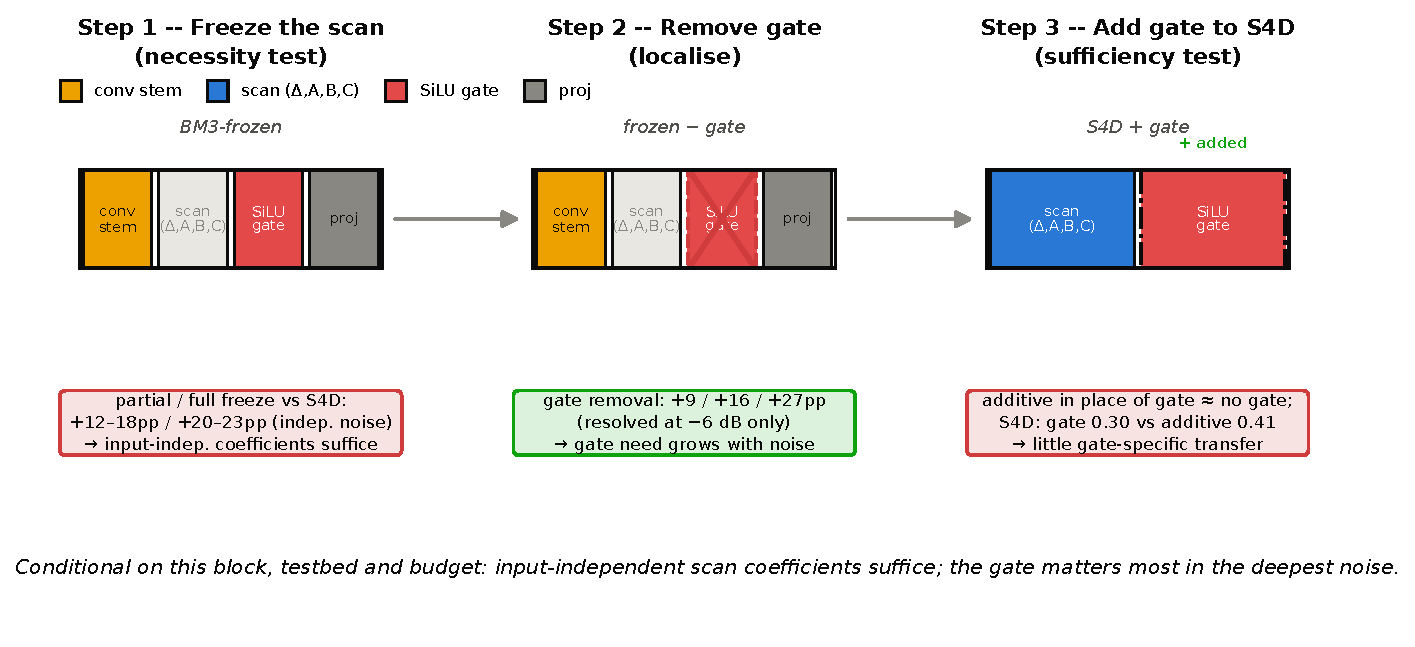
\includegraphics[width=0.85\linewidth]{figures/fig1_chain}
\caption{The three-step ablation chain with pre-specified thresholds: freeze the input-dependent $\Delta,A,B,C$ projections (Section~\ref{sec:results:falsify}), remove one component at a time on the frozen base to localise the necessary ingredient (Section~\ref{sec:results:localise}), and graft that ingredient onto S4D to test sufficiency (Section~\ref{sec:results:graft}).}
\label{fig:chain}
\end{figure}

\subsection{Freezing the input-dependent $\Delta$, $A$, $B$, $C$ projections}
\label{sec:results:falsify}

\begin{table}[htbp]
\centering
\caption{BM3 vs.\ BM3-frozen vs.\ S4D, macro-F1 (\%) by SNR (frozen-selectivity grid). $\Delta$(BM3$-$frozen) and $\Delta$(frozen$-$S4D) in percentage points.}
\label{tab:falsify}
\begin{tabular}{@{}lrrrrr@{}}
\toprule
Condition & BM3 & BM3-frozen & S4D & $\Delta$(BM3$-$frozen) & $\Delta$(frozen$-$S4D) \\
\midrule
clean & 78.9 & 78.9 & 81.0 & $-0.0$ & $-2.1$ \\
0\,dB & 95.0 & 89.9 & 76.1 & $+5.1$ & $\mathbf{+13.8}$ \\
$-2$\,dB & 95.4 & 92.1 & 75.1 & $+3.3$ & $\mathbf{+17.0}$ \\
$-6$\,dB & 88.5 & 86.3 & 68.5 & $+2.2$ & $\mathbf{+17.7}$ \\
$-10$\,dB\rlap{$^{*}$} & 68.1 & 64.3 & 52.3 & $+3.8$ & $+12.0$ \\
\bottomrule
\end{tabular}
\end{table}

\begin{figure}[htbp]
\centering
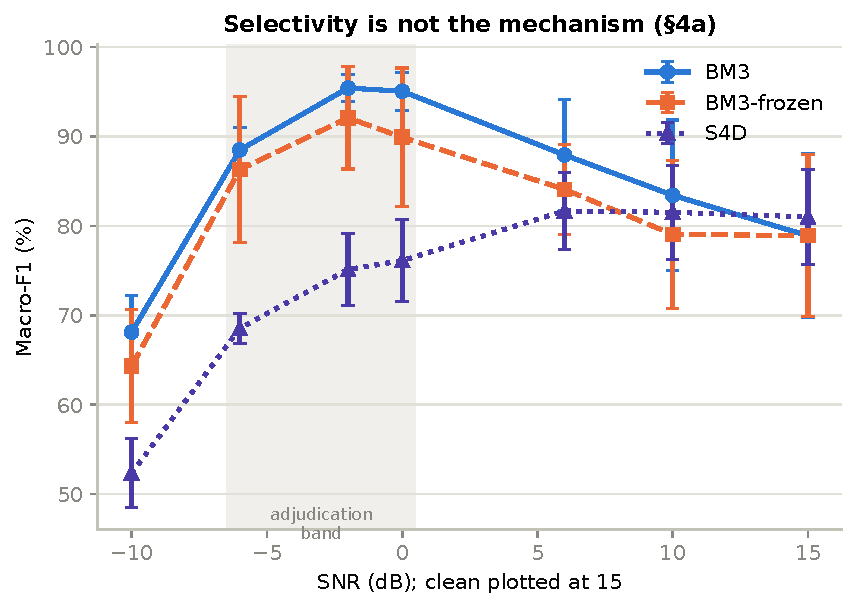
\includegraphics[width=0.85\linewidth]{figures/fig2_snr_curves}
\caption{Macro-F1 vs.\ SNR for BM3, BM3-frozen, and S4D across the full noise grid. The frozen arm tracks BM3 closely and stays well above S4D throughout the adjudication band.}
\label{fig:snr_curves}
\end{figure}

Freezing the input-dependent $\Delta$, $A$, $B$, $C$ projections (Section~\ref{sec:protocol:freeze}) costs at most $5.1\pp$ anywhere in the adjudication band on the point estimates, while the frozen block retains a $13.8$--$17.7\pp$ advantage over S4D (Table~\ref{tab:falsify}, Figure~\ref{fig:snr_curves}). Five seeds bound these quantities loosely: paired 95\% intervals for $\Delta$(BM3$-$frozen) are $[-4.7, 15.0]$, $[-3.1, 9.8]$ and $[-7.5, 11.8]\pp$ at $0$, $-2$ and $-6$\,dB (BM3 ahead in 3/5, 4/5 and 2/5 seeds), and for $\Delta$(frozen$-$S4D) $[-0.5, 28.0]$, $[5.5, 28.4]$ and $[5.8, 29.7]\pp$ (5/5, 5/5, 5/5 seeds). The pre-specified rule attributed robustness to selectivity only if $\Delta$(BM3$-$frozen) $\geq 10\pp$ in deep noise with the frozen arm collapsing toward S4D. Neither condition holds on the point estimates, so the pre-specified verdict is that these projections are \emph{not the primary mechanism}. This is a failure to meet a confirmation criterion, not a demonstration that freezing is cheap: the intervals above are compatible with differences larger than $10\pp$, and no equivalence margin was pre-specified or tested. One limit applies: the frozen arm still contains input-dependent trapezoidal weights and rotation angles, so this result concerns $\Delta, A, B, C$ only; Section~\ref{sec:results:fullfreeze} removes that limit. Under last-epoch reporting the re-run gives $\Delta$(BM3$-$frozen) $= +3.7$, $+0.9$ and $+0.2\pp$ (best-epoch re-run: $+5.1$, $+3.5$, $+3.0\pp$; intervals still include zero at every level), so the point estimates fall further below the $10\pp$ threshold rather than rising towards it. On clean data S4D matches or slightly exceeds both Mamba-style arms---consistent with the systematic clean-TSC comparison~\cite{saadatmand2026s4d}. In the noisy regime, the block's advantage over S4D is not removed by freezing these four terms, so it must be carried by other parts of the block or by the remaining input-dependent scan terms.

\subsection{Freezing the remaining input-dependent scan terms}
\label{sec:results:fullfreeze}

Table~\ref{tab:fullfreeze} reports the three layered arms of Section~\ref{sec:protocol:freeze} on the adjudication band (60 cells: 4 arms $\times$ 3 levels $\times$ 5 seeds $\times$ 50 epochs, the original training code, the same evaluation fingerprint, with the original BM3 arm re-run in the same grid). The question is whether the advantage that survived freezing $\Delta, A, B, C$ is carried by the two input-dependent terms the frozen arm retained.

\begin{table}[htbp]
\centering
\caption{Layered freezing of the scan's input-dependent terms. Macro-F1 (\%), mean over 5 seeds, under best-epoch and final-epoch reporting; $\Delta$ columns are paired differences under final-epoch reporting with 95\% $t$-intervals over seeds.}
\label{tab:fullfreeze}
\footnotesize\setlength{\tabcolsep}{4pt}
\begin{tabular}{@{}lrrrrrr@{}}
\toprule
 & \multicolumn{2}{c}{0\,dB} & \multicolumn{2}{c}{$-2$\,dB} & \multicolumn{2}{c}{$-6$\,dB} \\
\cmidrule(lr){2-3}\cmidrule(lr){4-5}\cmidrule(lr){6-7}
Arm & best & final & best & final & best & final \\
\midrule
BM3 (re-run) & 95.6 & 86.9 & 95.8 & 88.3 & 88.6 & 83.3 \\
BM3-frozen ($\Delta,A,B,C$) & 90.6 & 83.1 & 92.3 & 87.3 & 85.7 & 83.1 \\
frozen$-$trap & 95.5 & 87.6 & 95.3 & 89.3 & 90.5 & 88.0 \\
frozen$-$rot & 94.6 & 86.7 & 94.6 & 89.1 & 89.0 & 86.4 \\
frozen$-$all & 96.5 & 89.5 & 96.8 & 91.5 & 90.5 & 87.9 \\
S4D & 75.9 & 67.6 & 75.1 & 67.5 & 68.6 & 66.7 \\
\midrule
\multicolumn{7}{@{}l}{\emph{Paired differences, final-epoch reporting (pp)}} \\
frozen$-$all $-$ S4D & \multicolumn{2}{c}{$+21.9$ [16.7, 27.1]} & \multicolumn{2}{c}{$+24.0$ [21.4, 26.5]} & \multicolumn{2}{c}{$+21.2$ [17.5, 24.9]} \\
BM3-frozen $-$ frozen$-$all & \multicolumn{2}{c}{$-6.3$ [$-$17.6, 4.9]} & \multicolumn{2}{c}{$-4.1$ [$-$12.0, 3.7]} & \multicolumn{2}{c}{$-4.8$ [$-$17.8, 8.2]} \\
BM3 $-$ frozen$-$all & \multicolumn{2}{c}{$-2.6$ [$-$8.2, 2.9]} & \multicolumn{2}{c}{$-3.2$ [$-$7.0, 0.6]} & \multicolumn{2}{c}{$-4.5$ [$-$7.2, $-$1.9]} \\
\bottomrule
\end{tabular}
\end{table}

It is not. With every tensor entering the scan input-independent, \emph{frozen$-$all} is $+21.9$, $+24.0$ and $+21.2\pp$ above S4D at $0$, $-2$ and $-6$\,dB under final-epoch reporting, positive in 5/5 seeds at every level and with intervals excluding zero---if anything a larger margin than the partially frozen arm's $+15.5$, $+19.8$, $+16.4\pp$ (Table~\ref{tab:sensitivity_contrasts}). None of the three freezing steps costs accuracy: the paired differences BM3-frozen $-$ frozen$-$trap, $-$ frozen$-$rot and $-$ frozen$-$all are negative at all three levels (between $-1.8$ and $-6.3\pp$ under final-epoch reporting), i.e.\ the more heavily frozen arm is numerically ahead, with every interval including zero. The direction is not an artefact of capacity: \emph{frozen$-$all} has 103{,}842 parameters against 112{,}410 for BM3-frozen and 177{,}938 for BM3. At the deepest level \emph{frozen$-$all} also exceeds the full BM3 block by $4.5\pp$ ($[-7.2, -1.9]$ for BM3 $-$ frozen$-$all, 0/5 seeds in BM3's favour); we report this but do not build on it, since five seeds and one speed pair cannot separate a genuine advantage of a time-invariant scan from a variance effect.

Two readings of the whole step are therefore available, and the data do not separate them: input-dependence of the scan contributes nothing measurable here, or it contributes something that the learned constants recover under this training budget. Either way the conclusion for the attribution chain is the same and now rests on a complete intervention rather than a partial one: \textbf{the Mamba-style block's deep-noise advantage over a time-invariant S4D does not require any input-dependent term in its scan}. What remains to carry it is the rest of the block---the convolutional stem, the heavy-tailed $A$ parameterisation, the normalisations and the output gate---which is what Sections~\ref{sec:results:localise}--\ref{sec:results:graft} examine. The re-run also reproduces the original grids: the BM3 arm's best-epoch means (95.6, 95.8, 88.6) exceed Table~\ref{tab:falsify}'s 95.0, 95.4, 88.5 by $0.57$, $0.43$ and $0.16\pp$ (a different PyTorch/Triton build, Section~\ref{sec:results:sensitivity}).

\subsection{Removing the gate is the only ablation with a large, one-signed effect}
\label{sec:results:localise}

\begin{table}[htbp]
\centering
\caption{Single-component removal on the frozen base (component-ablation grid, trained separately from Table~\ref{tab:falsify}), $\Delta$(frozen $-$ arm) in percentage points.}
\label{tab:localise}
\begin{tabular}{@{}lrrrp{4.0cm}@{}}
\toprule
Component removed & 0\,dB & $-2$\,dB & $-6$\,dB & Adjudication \\
\midrule
SiLU gate & $\mathbf{+13.1}$ & $\mathbf{+21.1}$ & $\mathbf{+23.5}$ & PRIMARY (all $\geq 8\pp$) \\
conv stem ($k{=}7$) & $-6.6$ & $-2.7$ & $+7.9$ & outside pre-specified bins (regime trade-off) \\
heavy-tailed $A \rightarrow$ S4D-style $A$ & $-2.4$ & $-2.2$ & $-4.2$ & outside bins (removal numerically beneficial; intervals include 0) \\
\bottomrule
\end{tabular}
\end{table}

\begin{figure}[htbp]
\centering
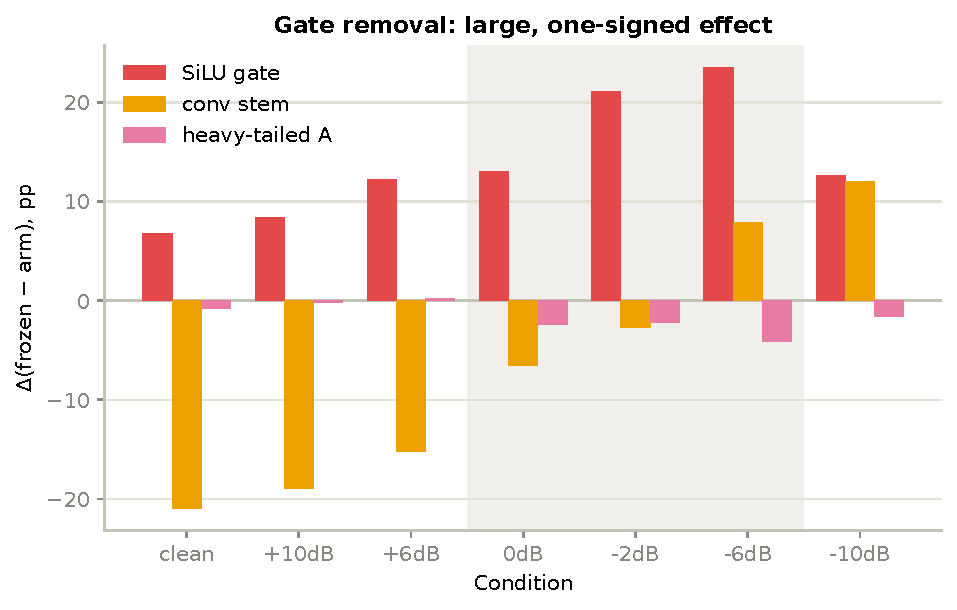
\includegraphics[width=0.85\linewidth]{figures/fig3_ablation_bars}
\caption{Component-removal $\Delta$ (percentage points, frozen $-$ arm) by SNR for the three single-component ablations on the frozen base. Only gate removal is monotone, large, and one-signed across the adjudication band.}
\label{fig:ablation_bars}
\end{figure}

``Necessary'' is used here in the operational sense of this ablation: removing the gate from the frozen block, with the other components and the budget unchanged, removes most of the block's advantage. The gate result is large, one-signed and monotone in noise depth: removal costs $13.1$, $21.1$ and $23.5\pp$ at $0$, $-2$ and $-6$\,dB (paired 95\% intervals $[6.5, 19.6]$, $[3.8, 38.5]$, $[8.5, 38.6]\pp$; 5/5 seeds at every level). The gateless arm also gives up most of the Mamba advantage: it sits \textbf{below plain S4D} at $-2$\,dB (71.7 vs.\ 75.2) and $-6$\,dB (62.5 vs.\ 68.6), though not at $0$\,dB (77.6 vs.\ 76.2), and the gateless--S4D gap itself is not resolved by five seeds (Section~\ref{sec:results:sensitivity}: under last-epoch reporting the gateless arm is below S4D at $-6$\,dB only). We read this as ``at best on par with S4D, and worse at the deepest noise level'', which suggests, but does not establish, that components interact rather than add. The other two components tell regime stories rather than robustness stories: the convolutional stem helps by $7.9\pp$ at $-6$\,dB (removal gives 78.1 vs.\ 86.0; paired 95\% interval of the difference $[-2.1, 17.9]\pp$, 4/5 seeds) but \emph{costs} $21.0\pp$ on clean cross-speed data (removal yields 98.8 vs.\ 77.8, with seed-std collapsing from $8.1$ to $0.6\pp$)---consistent either with speed-specific local temporal patterns mistransferring across conditions, or with optimisation friction under the matched budget; we report both readings. Replacing the heavy-tailed state parameterisation by an S4D-style one is numerically beneficial at all three deep-noise levels ($+2.4$, $+2.2$, $+4.2\pp$), but every paired interval includes zero (e.g., $[-15.4, 7.1]\pp$ at $-6$\,dB), so we draw no directional conclusion from it (numerically, the S4D-style variant is the best deep-noise cell in the component grid, 90.1 at $-6$\,dB).

\subsection{Adding a narrow gate branch to S4D}
\label{sec:results:graft}

\begin{table}[htbp]
\centering
\caption{Grafting the SiLU gate branch onto plain S4D (S4D unchanged key-by-key; only the gate branch added). The S4D+gate column is the graft grid; the S4D and BM3-frozen columns, and hence $R$, are the component-ablation grid of Section~\ref{sec:results:localise}, as pre-specified, which is why they differ from Table~\ref{tab:falsify} by 0.1--0.7\,pp (independent runs of the same arms).}
\label{tab:graft}
\begin{tabular}{@{}lrrrr@{}}
\toprule
Condition & S4D+gate & S4D & BM3-frozen & Recovery ratio \\
\midrule
0\,dB & 79.8 & 76.2 & 90.6 & 0.249 \\
$-2$\,dB & 79.4 & 75.2 & 92.8 & 0.239 \\
$-6$\,dB & 69.2 & 68.6 & 86.0 & $\mathbf{0.035}$ \\
\bottomrule
\end{tabular}
\end{table}

\begin{figure}[htbp]
\centering
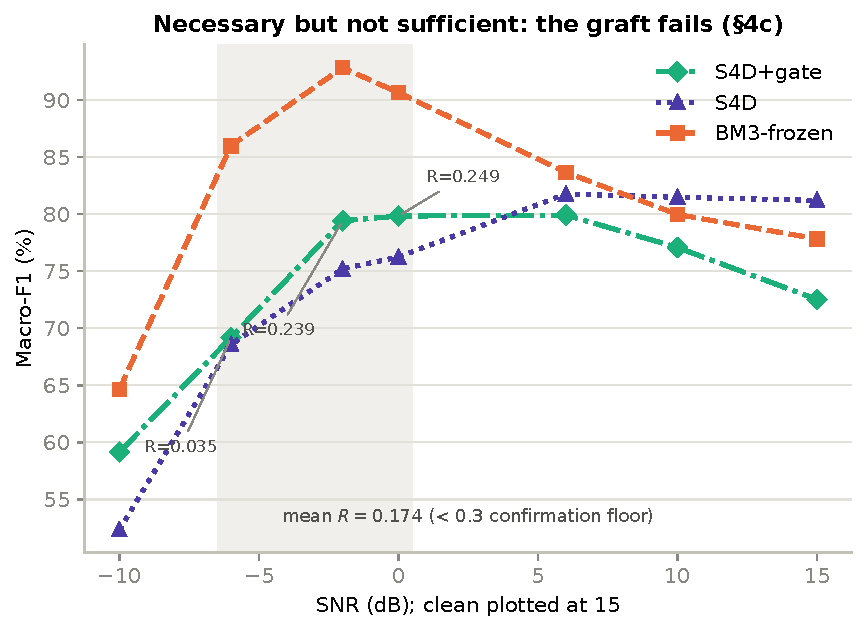
\includegraphics[width=0.85\linewidth]{figures/fig4_graft}
\caption{Graft outcome: S4D+gate, plain S4D, and BM3-frozen across the adjudication band, with the per-condition recovery ratio $R = (\text{S4D+gate} - \text{S4D})/(\text{frozen} - \text{S4D})$ annotated. Recovery is near zero at the deepest adjudicated noise level. This is the narrow graft; the width-matched graft and its additive control are in Table~\ref{tab:graftwm}.}
\label{fig:graft}
\end{figure}

Pre-specified recovery ratio $R = $ mean over the band of $(\text{S4D+gate} - \text{S4D})/(\text{frozen} - \text{S4D}) = \mathbf{0.174}$. The pre-specified bins were $R \geq 0.7$ (confirmed), $0.3 \leq R < 0.7$ (partial recovery) and $R < 0.3$ (insufficient); $R = 0.174$ falls in the last. Resampling seeds within each arm gives a 95\% interval of $[0.04, 0.29]$ for $R$, and the per-level paired gains of S4D+gate over S4D are $+3.6$ ($[-2.2, 9.3]$), $+4.2$ ($[1.1, 7.3]$) and $+0.6\pp$ ($[-2.2, 3.4]$). At the deepest adjudicated level the graft recovers essentially nothing. Removal and addition are not mirror-image interventions. In BM3 the gate has its own $64 \rightarrow 128$ projection and multiplies the scan output at the inner width of 128 before the output projection; removing it deletes $32{,}768$ parameters. In the S4D host the grafted gate is a $64 \rightarrow 64$ linear branch (with bias) computed from the layer input and multiplying the SSM output before the residual addition; it adds $16{,}640$ parameters over four layers. The two share the multiplicative SiLU form but not width, projection structure or parameter count. Removal costs $13$--$24\pp$ in the frozen block whereas this graft adds $0.6$--$4.2\pp$ to S4D. What this shows is that \emph{this gate branch, in this host and under this budget, recovers little}. Three readings fit the data and cannot be separated here: (i) host dependence, i.e.\ the gate needs the stem or scan context it co-trained with; (ii) implementation differences in width, projection and placement; (iii) transplant friction, i.e.\ the grafted branch is harder to optimise in a foreign host under the matched budget (training converges normally, but convergence is not robustness). Section~\ref{sec:results:graftwm} tests reading (ii) with a width-matched graft and an equal-capacity non-multiplicative control; a tuning or longer-budget comparison selected on a source-domain validation set was not run.

The four arms do allow a coarse host-by-gate contrast, $I = [F(\text{frozen}) - F(\text{frozen}{-}\text{gate})] - [F(\text{S4D+gate}) - F(\text{S4D})]$, where $F$ is macro-F1. Under last-epoch reporting $I = 5.2$ $[2.3, 8.1]$, $8.9$ $[-6.2, 23.9]$ and $22.6$ $[2.9, 42.4]\pp$ at $0$, $-2$ and $-6$\,dB (seed-matched 95\% $t$-intervals; positive in 5/5, 4/5 and 5/5 seeds); under best-epoch reporting in the re-run it is $7.8$ $[1.4, 14.2]$, $14.4$ $[-1.4, 30.3]$ and $23.1$ $[8.7, 37.4]\pp$. A positive $I$ means the gate adds more on the frozen host than on S4D. Because the host differs in several respects at once and the two gates are not aligned, $I$ cannot be assigned to a specific component or interaction term, and the seed pairing across arms is nominal (arms share seed indices, not initialisations).

\subsection{A width-matched graft and an additive control}
\label{sec:results:graftwm}

The graft of Section~\ref{sec:results:graft} is narrower and smaller than the donor gate. Two further arms rebuild it in the donor's shape (Table~\ref{tab:arms}). In each layer the layer input is projected to $x$ and $z$ of width 128 (the frozen block's inner width), the S4D layer runs on $x$ at width 128 with state size 64---so that its own parameter count and total state size equal the host's 64-wide, state-128 layer---and an output projection maps back to width 64. \emph{S4D+gate (wm)} combines $y \odot \mathrm{SiLU}(z)$, as the donor does; \emph{S4D+branch} uses the same modules, parameters and initial weights but combines $y + \mathrm{SiLU}(z)$. Both have 198{,}978 parameters, more than BM3-frozen (112{,}410) and BM3 (177{,}938), which biases the test towards recovery. A construction check with forward hooks confirms that the tensor entering the output projection equals the intended formula for each arm and not the other, and that the two arms are identical at initialisation. The thresholds were committed publicly before the grid ran (Section~\ref{sec:protocol:prereg}): $R$ as before, under final-epoch reporting; the verdict is INCONCLUSIVE whenever the seed-resampled interval crosses a bin boundary, in which case we write at the tier less favourable to the claim; and a gate-specific reading requires $\Delta R = R_{\text{gate}} - R_{\text{branch}} > 0.1$ with an interval excluding zero.

\begin{table}[htbp]
\centering
\caption{Width-matched graft and additive control on the original transition. Macro-F1 (\%), mean over 5 seeds, final-epoch reporting; $R$ is the mean over the three levels of (arm $-$ S4D)/(BM3-frozen $-$ S4D), with a seed-resampled 95\% interval. S4D, BM3-frozen and the narrow graft are the re-runs of Section~\ref{sec:results:sensitivity}.}
\label{tab:graftwm}
\footnotesize
\begin{tabular}{@{}lrrrcc@{}}
\toprule
Arm & 0\,dB & $-2$\,dB & $-6$\,dB & $R$ & 95\% interval \\
\midrule
S4D & 67.6 & 67.5 & 66.7 & -- & -- \\
S4D+gate (narrow) & 71.5 & 74.3 & 66.6 & 0.196 & [0.09, 0.31] \\
S4D+gate (wm) & 70.1 & 73.4 & 73.8 & 0.296 & [0.16, 0.52] \\
S4D+branch & 73.1 & 76.2 & 73.8 & 0.408 & [0.31, 0.60] \\
BM3-frozen & 83.1 & 87.3 & 83.1 & 1 & -- \\
\midrule
\multicolumn{4}{@{}l}{$\Delta R$ = S4D+gate (wm) $-$ S4D+branch} & $-0.112$ & [$-$0.26, 0.02] \\
\bottomrule
\end{tabular}
\end{table}

The width-matched graft recovers $R = 0.296$ of the gap (per level 0.159, 0.298, 0.431). Its interval, $[0.16, 0.52]$, crosses the 0.3 boundary, so the pre-specified verdict is INCONCLUSIVE between ``insufficient'' and ``partial'', and we report it at the less favourable tier: a graft built in the donor's shape recovers part of the gap. The recovery is not gate-specific. The additive branch, with the same parameters, recovers at least as much ($R = 0.408$), $\Delta R = -0.112$ $[-0.26, 0.02]$, and at 0\,dB the gated arm is below the additive one by $3.0\pp$ ($[-4.5, -1.5]$, 0/5 seeds). With frozen$-$all in the denominator the gated arm's ratio is $0.231$ $[0.13, 0.33]$; under best-epoch reporting the two ratios are 0.459 and 0.483. What a graft recovers on this transition therefore follows the added structure---a wider channel axis and input/output projections---rather than the multiplicative interaction. Reading (ii) of Section~\ref{sec:results:graft} is partly confirmed, in that the narrow graft understated what added structure can recover; but in the S4D host the gate itself contributes nothing beyond an equal-capacity additive branch, whereas removing it from the frozen Mamba-3 block costs $9$--$23\pp$ under the same rule (Table~\ref{tab:sensitivity_contrasts}).

\subsection{Replacing the gate in its native host}
\label{sec:results:nativeadd}

The previous subsection changes the host and keeps the operator. A pre-specified grid (15 cells, original transition) does the converse: it keeps the host and changes the operator. In \emph{frozen$+$add} the scan kernel of every BM3-frozen layer is called without gating and the layer output becomes $W_{\mathrm{out}}(y + \mathrm{SiLU}(z))$; modules, parameter count (112{,}410) and initial weights are bitwise those of BM3-frozen, and a construction check confirms that the donor operator is $y \odot \mathrm{SiLU}(z)$ and that the new arm computes $y + \mathrm{SiLU}(z)$. The pre-specified statistic is the native rescue ratio $\rho = (\text{add} - \text{no gate})/(\text{frozen} - \text{no gate})$, mean over levels, final epoch, with a seed-resampled interval; \emph{not rescued} requires $\rho < 0.3$ with an upper bound below $0.5$.

\begin{table}[htbp]
\centering
\caption{Gate replaced by an additive branch inside BM3-frozen (original transition). Macro-F1 (\%), mean over 5 seeds; paired differences under final-epoch reporting with 95\% $t$-intervals and the number of seeds (of 5) with a positive difference.}
\label{tab:nativeadd}
\footnotesize\setlength{\tabcolsep}{4pt}
\begin{tabular}{@{}lcccccc@{}}
\toprule
 & \multicolumn{2}{c}{0\,dB} & \multicolumn{2}{c}{$-2$\,dB} & \multicolumn{2}{c}{$-6$\,dB} \\
\cmidrule(lr){2-3}\cmidrule(lr){4-5}\cmidrule(lr){6-7}
Arm & best & final & best & final & best & final \\
\midrule
BM3-frozen ($y \odot \mathrm{SiLU}(z)$) & 90.6 & 83.1 & 92.3 & 87.3 & 85.7 & 83.1 \\
frozen$+$add ($y + \mathrm{SiLU}(z)$) & 78.0 & 74.7 & 72.6 & 71.5 & 62.3 & 60.9 \\
frozen$-$gate (no $z$) & 77.7 & 74.0 & 73.1 & 71.7 & 61.9 & 60.5 \\
\midrule
BM3-frozen $-$ frozen$+$add & \multicolumn{2}{c}{\shortstack{$+8.5$\\ {[}1.1, 15.9{]} (5/5)}} & \multicolumn{2}{c}{\shortstack{$+15.8$\\ {[}$-$1.2, 32.9{]} (4/5)}} & \multicolumn{2}{c}{\shortstack{$+22.2$\\ {[}4.6, 39.9{]} (5/5)}} \\[3pt]
frozen$+$add $-$ frozen$-$gate & \multicolumn{2}{c}{\shortstack{$+0.6$\\ {[}$-$1.7, 3.0{]} (3/5)}} & \multicolumn{2}{c}{\shortstack{$-0.2$\\ {[}$-$3.4, 3.0{]} (3/5)}} & \multicolumn{2}{c}{\shortstack{$+0.4$\\ {[}$-$0.7, 1.4{]} (3/5)}} \\[3pt]
\bottomrule
\end{tabular}
\end{table}

The additive branch rescues nothing. frozen$+$add is indistinguishable from the gateless arm at every level ($+0.6$, $-0.2$, $+0.4$\,pp, every interval including zero), and the multiplicative arm exceeds it by $8.5$, $15.8$, $22.2$\,pp. The rescue ratio is $\rho = 0.024$ (per level 0.070, $-$0.015, 0.016), with a seed-resampled 95\% interval of $[-1.159, 0.486]$; under best-epoch reporting $\rho = 0.005$. By the pre-specified rule the verdict is \emph{not rescued}. Two features of the interval should be read with it: its upper bound lies only $0.014$ below the threshold, and its lower bound is wide because the 0\,dB denominator is only $9.1\pp$ (in 7.8\% of resamples one level's denominator fell below $2\pp$ and was excluded, as pre-specified).

Together with Section~\ref{sec:results:graftwm} this gives the two halves of a symmetric test. In the S4D host the gate adds nothing beyond an additive branch of the same size; in the Mamba-3 host an additive branch of the same size adds nothing beyond removing the gate. The benefit of the gate is specific to the multiplicative operator \emph{in its native host}, and what transfers to the time-invariant host is the added structure, not the gating.

\subsection{The reverse transition}
\label{sec:results:reverse}

A pre-specified grid repeats the chain's central contrasts on the reverse transition, 40\,Hz/10\,kN $\rightarrow$ 37.5\,Hz/11\,kN (75 cells: frozen$-$all, BM3-frozen, frozen$-$gate, S4D and S4D+gate (wm), at three levels and five seeds; Section~\ref{sec:protocol:testbed} for the data). This direction is harder for the time-invariant model: on its evaluation set, predicting the majority class gives a macro-F1 of 46.8\% and uniform random guessing 41.5\%, and S4D sits close to those levels (Table~\ref{tab:reverse}).

\begin{table}[htbp]
\centering
\caption{Reverse transition (40\,Hz/10\,kN $\rightarrow$ 37.5\,Hz/11\,kN). Macro-F1 (\%), mean over 5 seeds, best-epoch and final-epoch reporting; paired differences under final-epoch reporting with 95\% $t$-intervals and the number of seeds (of 5) with a positive difference.}
\label{tab:reverse}
\footnotesize\setlength{\tabcolsep}{4pt}
\begin{tabular}{@{}lccc@{}}
\toprule
Arm (best / final) & 0\,dB & $-2$\,dB & $-6$\,dB \\
\midrule
frozen$-$all & 86.3 / 77.5 & 87.8 / 77.9 & 81.7 / 74.0 \\
BM3-frozen & 81.1 / 74.7 & 84.0 / 76.7 & 80.8 / 73.9 \\
S4D+gate (wm) & 79.0 / 72.9 & 80.5 / 73.9 & 78.5 / 72.2 \\
frozen$-$gate & 63.8 / 56.2 & 62.0 / 54.7 & 57.1 / 50.0 \\
S4D & 61.2 / 51.2 & 61.0 / 52.4 & 54.6 / 51.8 \\
\midrule
frozen$-$all $-$ S4D & \shortstack{$+26.3$\\ {[}21.5, 31.0{]} (5/5)} & \shortstack{$+25.6$\\ {[}21.1, 30.1{]} (5/5)} & \shortstack{$+22.2$\\ {[}18.8, 25.6{]} (5/5)} \\[3pt]
BM3-frozen $-$ frozen$-$gate & \shortstack{$+18.4$\\ {[}1.2, 35.6{]} (5/5)} & \shortstack{$+22.0$\\ {[}3.4, 40.6{]} (5/5)} & \shortstack{$+24.0$\\ {[}7.6, 40.3{]} (5/5)} \\[3pt]
frozen$-$gate $-$ S4D & \shortstack{$+5.0$\\ {[}$-$17.6, 27.7{]} (2/5)} & \shortstack{$+2.4$\\ {[}$-$19.2, 23.9{]} (2/5)} & \shortstack{$-1.8$\\ {[}$-$18.9, 15.3{]} (1/5)} \\[3pt]
S4D+gate (wm) $-$ S4D & \shortstack{$+21.7$\\ {[}15.4, 28.0{]} (5/5)} & \shortstack{$+21.5$\\ {[}17.0, 26.0{]} (5/5)} & \shortstack{$+20.5$\\ {[}15.7, 25.2{]} (5/5)} \\[3pt]
\bottomrule
\end{tabular}
\end{table}

The first two steps replicate. The fully input-independent scan exceeds S4D by $+26.3$, $+25.6$ and $+22.2\pp$ at $0$, $-2$ and $-6$\,dB, with intervals excluding zero and 5/5 seeds at every level, so by the pre-specified rule (at least two of three levels) the first step is replicated on the reverse transition. Removing the gate from BM3-frozen costs $18.4$, $22.0$ and $24.0\pp$, above the $8\pp$ threshold at all three levels, with intervals excluding zero and 5/5 seeds, and the gateless arm is indistinguishable from S4D (intervals include zero). On the third step, which the pre-specification treats as descriptive here, the width-matched graft recovers most of the gap, $R = 0.911$ $[0.82, 1.04]$ ($0.863$ with frozen$-$all in the denominator). A further pre-specified grid (15 cells) adds the same-size additive control in this direction: it reaches 67.8, 72.1, 68.4\% (final epoch) and recovers $R = 0.758$ $[0.66, 0.88]$. The gate arm exceeds it by $+5.1$, $+1.7$, $+3.8$\,pp (only the $-6$\,dB interval excludes zero), and the difference in recovery is $\Delta R = 0.153$ $[0.06, 0.26]$; under best-epoch reporting it shrinks to $0.037$ $[-0.1, 0.17]$. By the pre-specified descriptive labels this is \emph{unresolved}: in this direction the gate carries a small increment over the additive branch, whereas on the original transition it carried none ($\Delta R = -0.112$). Most of the reverse-direction recovery is therefore available to an additive branch of the same size, and the remaining gate increment is direction-dependent. Both ratios rest on an S4D baseline close to the trivial floor (51--52\% against 46.8\% for the majority class). Both statements carry the limits of this pair: the same eight bearings with their roles swapped, and a single inner-race bearing in the evaluation set.

\subsection{Sensitivity to the reporting rule}
\label{sec:results:sensitivity}

The tables above use best-epoch macro-F1 on the evaluation condition (Section~\ref{sec:protocol:report}). To measure how much this rule shapes the conclusions, we re-ran the four arms that carry the chain (BM3-frozen, S4D, frozen$-$gate, S4D+gate) over the adjudication band: 60 cells, 5 seeds, 50 epochs, the original training code and the same evaluation fingerprint, recording macro-F1 at every epoch and reporting it at the final epoch, where the cosine learning-rate schedule has annealed to zero. This rule uses no evaluation data to pick a model. The re-run used a different PyTorch/Triton build from the original grids; its best-epoch values reproduce the original arm-by-condition means to within $-0.6$ to $+1.4\pp$ (the largest deviation is in the high-variance frozen$-$gate arm at $-2$\,dB). The S4D-wide capacity control and the conv-stem and $A$-parameterisation ablations were not re-run; the original BM3 arm was re-run in the stage-2 grid of Section~\ref{sec:results:fullfreeze}, so $\Delta$(BM3$-$frozen) is available under both rules.

\begin{table}[htbp]
\centering
\caption{Macro-F1 (\%), mean over 5 seeds, under best-epoch reporting (re-run) and final-epoch reporting.}
\label{tab:sensitivity_means}
\begin{tabular}{@{}lrrrrrr@{}}
\toprule
 & \multicolumn{2}{c}{0\,dB} & \multicolumn{2}{c}{$-2$\,dB} & \multicolumn{2}{c}{$-6$\,dB} \\
\cmidrule(lr){2-3}\cmidrule(lr){4-5}\cmidrule(lr){6-7}
Arm & best & final & best & final & best & final \\
\midrule
BM3-frozen & 90.6 & 83.1 & 92.3 & 87.3 & 85.7 & 83.1 \\
S4D & 75.9 & 67.6 & 75.1 & 67.5 & 68.6 & 66.7 \\
frozen$-$gate & 77.7 & 74.0 & 73.1 & 71.7 & 61.9 & 60.5 \\
S4D+gate & 80.9 & 71.5 & 79.9 & 74.3 & 69.2 & 66.6 \\
\bottomrule
\end{tabular}
\end{table}

Final-epoch values are lower than best-epoch values by $1.4$--$9.5\pp$ across the twelve arm-by-level means, so the absolute levels in Tables~\ref{tab:falsify}--\ref{tab:graft} are optimistic. The reduction is of similar size for the arms being contrasted (e.g., BM3-frozen $-7.4$, $-5.0$, $-2.6\pp$ and S4D $-8.3$, $-7.6$, $-1.9\pp$ at $0$, $-2$, $-6$\,dB), and the contrasts that carry the argument are correspondingly stable (Table~\ref{tab:sensitivity_contrasts}).

\begin{table}[htbp]
\centering
\caption{Paired differences under final-epoch reporting, in percentage points: mean, 95\% $t$-interval over seeds, and number of seeds (of 5) with a positive difference.}
\label{tab:sensitivity_contrasts}
\footnotesize\setlength{\tabcolsep}{4pt}
\begin{tabular}{@{}lccc@{}}
\toprule
Contrast & 0\,dB & $-2$\,dB & $-6$\,dB \\
\midrule
BM3-frozen $-$ S4D & \shortstack{$+15.5$\\ {[}4.3, 26.8{]} (5/5)} & \shortstack{$+19.8$\\ {[}12.0, 27.7{]} (5/5)} & \shortstack{$+16.4$\\ {[}4.1, 28.7{]} (4/5)} \\[3pt]
BM3-frozen $-$ frozen$-$gate & \shortstack{$+9.1$\\ {[}2.9, 15.3{]} (5/5)} & \shortstack{$+15.6$\\ {[}$-$0.8, 32.0{]} (4/5)} & \shortstack{$+22.6$\\ {[}5.8, 39.4{]} (5/5)} \\[3pt]
frozen$-$gate $-$ S4D & \shortstack{$+6.4$\\ {[}$-$2.9, 15.8{]} (4/5)} & \shortstack{$+4.2$\\ {[}$-$14.5, 22.9{]} (3/5)} & \shortstack{$-6.2$\\ {[}$-$23.5, 11.2{]} (1/5)} \\[3pt]
S4D+gate $-$ S4D & \shortstack{$+3.9$\\ {[}$-$0.8, 8.6{]} (4/5)} & \shortstack{$+6.8$\\ {[}2.4, 11.1{]} (5/5)} & \shortstack{$-0.1$\\ {[}$-$4.0, 3.9{]} (2/5)} \\[3pt]
\bottomrule
\end{tabular}
\end{table}

\emph{Selectivity.} The frozen block's advantage over S4D is $+15.5$, $+19.8$ and $+16.4\pp$ (and $+21.9$, $+24.0$, $+21.2\pp$ for the fully frozen scan, Section~\ref{sec:results:fullfreeze}), versus $+14.6$, $+17.2$ and $+17.1\pp$ under best-epoch reporting in the re-run. It remains positive in 5/5, 5/5 and 4/5 seeds, with intervals excluding zero at every level. \emph{Gate.} Removing the gate costs $9.1$, $15.6$ and $22.6\pp$ ($12.8$ to $23.8\pp$ under best-epoch reporting in the re-run), above the $8\pp$ pre-specified threshold at every level; the interval at $-2$\,dB includes zero ($[-0.8, 32.0]\pp$, 4/5 seeds) because of the large seed variance of the gateless arm (standard deviation $14.6\pp$ at $-2$\,dB). \emph{Gateless versus S4D.} Under final-epoch reporting the gateless arm is not below S4D at $0$ and $-2$\,dB (point estimates $+6.4$ and $+4.2\pp$) and is below it at $-6$\,dB ($-6.2\pp$); all three intervals include zero. The statement that gate removal ``falls below S4D'' is therefore supported only as a point-estimate observation at the deepest level, and we phrase it as ``to or below'' elsewhere. \emph{Graft.} The recovery ratio is $0.249$, $0.341$ and $-0.003$ per level and $R = 0.196$ on average (best-epoch re-run: $0.220$), again in the pre-specified ``insufficient'' bin on the point estimate. The seed-resampled 95\% interval is $[0.09, 0.31]$ and so reaches the $0.3$ boundary: with five seeds the data support ``far below confirmation ($0.7$) and probably below $0.3$'', not a precise value of $R$. The graft gain over S4D is resolved at $-2$\,dB only ($+6.8\pp$, $[2.4, 11.1]$) and is indistinguishable from zero at $-6$\,dB.

Because the final epoch of the same evaluation condition has been inspected repeatedly during this study, last-epoch values are also not a fresh confirmatory test. The reporting rule therefore changes absolute levels and the strength of the gateless-versus-S4D statement, but not the ordering BM3-frozen $>$ \{S4D+gate, frozen$-$gate, S4D\}, the size of the frozen block's advantage over S4D, or the verdicts of the pre-specified gate and graft rules.

\subsection{The interaction effect concentrates on the hard class}
\label{sec:results:perclass}

\begin{figure}[htbp]
\centering
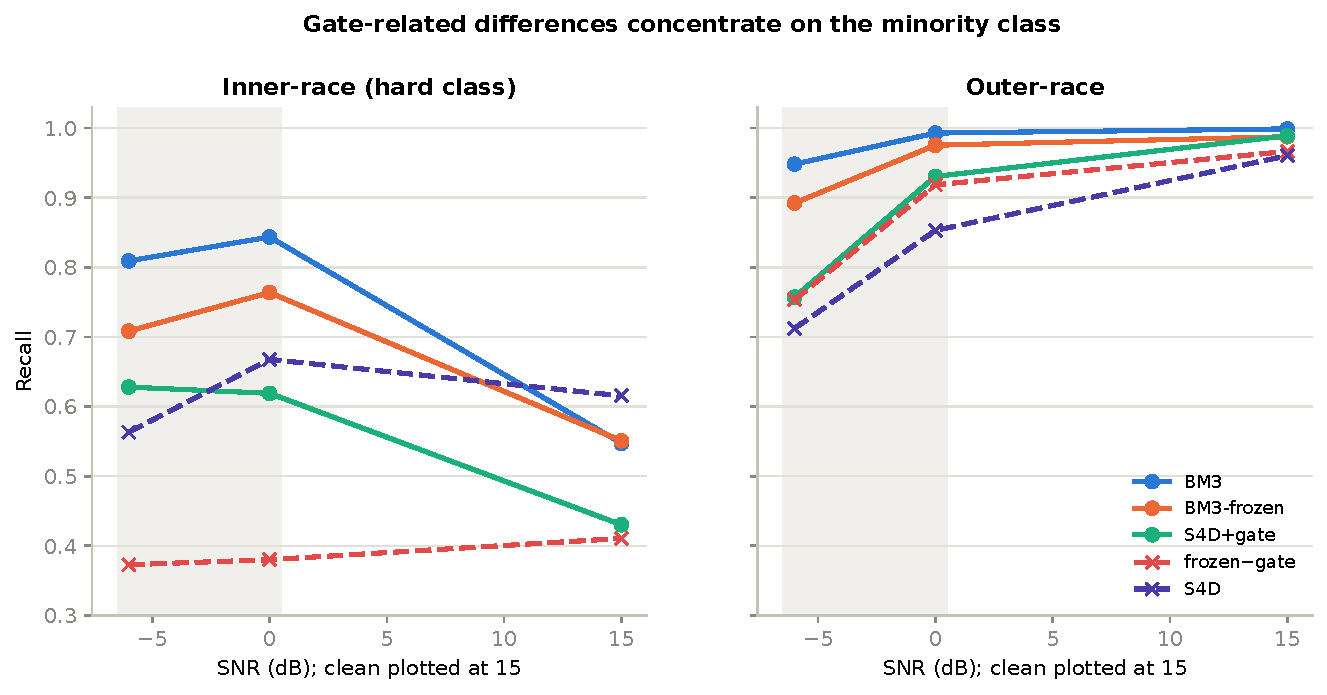
\includegraphics[width=0.85\linewidth]{figures/fig5_perclass}
\caption{Per-class recall (inner-race, IR, and outer-race, OR) as a function of noise depth, split by gate presence. Gated arms lift IR recall under matched noise; gateless arms let it deteriorate.}
\label{fig:perclass}
\end{figure}

Per-class analysis (a separate 75-cell grid at 20 epochs with best-epoch selection on the evaluation condition: 5 arms $\times$ $\{$clean, 0, $-6\,\mathrm{dB}\}$ $\times$ 5 seeds, per-sample predictions dumped and re-verified against reported metrics cell-by-cell): the inner-race class is hard from the outset (clean recall $0.41$--$0.62$ vs.\ $0.96$--$1.00$ for outer-race). Its trajectory under noise is governed by gate presence: in all three gated arms IR recall at $-6$\,dB exceeds its clean value (e.g., $0.55 \rightarrow 0.81$ for BM3), while in both gateless arms it is below its clean value (frozen$-$gate: $0.41 \rightarrow 0.37$; S4D: $0.62 \rightarrow 0.56$, non-monotone, rising to $0.67$ at $0$\,dB) (Figure~\ref{fig:perclass}). Both ablation directions hit IR hardest---gate removal costs IR $2.3$--$3.8\times$ more F1 than OR at every level (F1 from predictions pooled over seeds), and the graft's noise-time gains also concentrate on IR ($-6$\,dB: $+6.8\pp$ IR vs.\ $+4.2\pp$ OR). Because macro-F1 averages the two classes, the arm-level robustness gaps of Sections~\ref{sec:results:falsify}--\ref{sec:results:graft} are carried substantially by the hard class. The gate-related differences are therefore class-concentrated rather than uniform, and fall on the class with the lowest recall. We did not measure classification margins, so we do not describe IR as a ``low-margin'' class. Because this grid is separate from the main 50-epoch grid and the IR class comes from a single training bearing (Section~\ref{sec:protocol:testbed}), these results are descriptive and do not decompose the main-grid effects.

\section{Discussion}
\label{sec:discussion}

\textbf{What should be credited?} The three-step chain licenses a specific, narrow attribution: within this block, on this testbed, deep-noise robustness is earned by the composition---gate $\times$ (stem, scan, parameterisation)---with the gate as the necessary but non-transplantable ingredient, and with selectivity, capacity, normalisation and the physics loss all eliminated as explanations. The apparent contradiction between ``selectivity makes Mamba robust'' narratives and S4D-superiority findings~\cite{saadatmand2026s4d} dissolves under this credit assignment: both literatures are right in their regimes, and neither regime is about selectivity.

\textbf{Implications for backbone selection and for transplant practice.} For practitioners choosing backbones for noisy, drifting signal regimes: what a Mamba-style block buys is its composition, and its cost structure should be judged accordingly (the gate cannot be cherry-picked into a cheaper host; our graft numbers quantify the failure). For the growing practice of porting Mamba components into CNNs, Transformers, or hybrid diagnosis models with an expectation of robustness gains, Section~\ref{sec:results:graft} is a directly usable negative result. A falsifiable engineering prediction follows: a recomposed block guided by the component map (no conv stem, gate retained, S4D-style $A$) should dominate the original on this testbed; we deliberately leave this untested here, as post-hoc recomposition after seeing the map would not carry the evidential status of the preregistered chain.

\textbf{Why might gating be composition-bound?} We refrain from a mechanistic claim beyond the data, but note three compatible observations. First, the gate's benefit concentrates on the low-margin class (Section~\ref{sec:results:perclass}), and matched-noise training lifts that class \emph{only when the gate is present}---suggesting the gate is the component through which matched-noise training is converted into hard-class margin, i.e., an exploiter of noise-aware training rather than a test-time denoiser (this reading is bounded by the matched-SNR scope, Section~\ref{sec:boundaries}). Second, its role appears closer to adaptive per-sample feature suppression than to generic denoising. Third, the gateless composition falling \emph{below} S4D indicates the other components are calibrated to a gated regime (e.g., the stem may pass features that are only safe when the gate can veto them). All are testable in future work via pairwise interaction grids and mismatched-noise protocols.

\section{Boundaries and Limitations}
\label{sec:boundaries}

We state the scope plainly.

\begin{enumerate}
\item \textbf{Testbed scope.} All claims are bounded to bearing vibration from one pair of operating conditions of one dataset (37.5\,Hz/11\,kN and 40\,Hz/10\,kN; speed and load both change), binary classification, GPU execution (no edge/real-time claims). Within each direction the training and evaluation bearings are disjoint; the reverse direction uses the same eight bearings with their roles swapped, has a single IR bearing in its evaluation set (the forward direction a single IR bearing in its training set) and so tests direction rather than new bearings; the third condition of the dataset has no IR bearing. The seeds do not resample bearings (Section~\ref{sec:protocol:testbed}), so the intervals carry no bearing-level uncertainty. Further independent datasets and multi-class settings are future work.
\item \textbf{Attribution level.} Credit assigned to ``the rest of the composition'' is by elimination within the enumerated component set; pairwise interaction terms are not decomposed.
\item \textbf{Transplant results are earlier-protocol and budget-conditional.} The graft onto S4D was run only under the earlier noise protocol, with a matched 50-epoch budget; a longer or graft-tuned budget might recover more, and we make no claim beyond \emph{this gate branch, in this host, under a matched training budget} (\ref{sec:results:graft}).
\item \textbf{Matched-SNR scope.} Training and evaluation share the same injected SNR throughout (Section~\ref{sec:protocol:testbed}); ``robustness'' in this paper is matched-noise robustness under noise-aware training, not clean-train/noisy-test generalisation. The gate's benefit may operate by exploiting matched-noise training (consistent with \ref{sec:results:perclass}) rather than by test-time denoising; attribution under mismatched-noise protocols is untested and may differ.
\item \textbf{Coverage by protocol.} Table~\ref{tab:coverage} states which operations were run under independent noise. Not run under independent noise: the graft onto S4D, the stem and $A$ ablations, additive substitution on the reverse transition, the per-class grid and the disjoint-bearing Paderborn setting. Not run at all: gate removal and additive substitution in the fully frozen block on the reverse transition, and the fully frozen block, additive arm and graft on Paderborn shared bearings.
\item \textbf{Noise-regime coverage.} Under strong coloured noise at $-10$\,dB a TCN baseline slightly overtakes the Mamba-style block, and $-10$\,dB is near-chance for the time-invariant baseline and excluded from adjudication; the demonstrated advantage regime is matched, Gaussian-dominated noise.
\item \textbf{Conv-stem dual reading.} Its clean-data cost admits both representation-mistransfer and optimisation-difficulty readings, reported in place (\ref{sec:results:localise}).
\item \textbf{Reporting rule.} Reported values are final-epoch macro-F1 under a fixed 50-epoch budget. The best-epoch rule of the original grids, for which the early thresholds were pre-specified, is optimistic by $0.6$--$10.6\pp$ (\ref{sec:results:sensitivity}). The final-epoch re-run of the original-design arms (earlier noise protocol) and the independent-noise re-run cover different sets of cells (Table~\ref{tab:coverage}); levels outside the adjudication band and the per-class grid were not re-run. No source-domain validation rule was available, and because the final epoch of the same evaluation condition has been inspected repeatedly, final-epoch values are not a fresh confirmatory test.
\item \textbf{Scope of the freezing intervention.} The first freeze arm removes the input-dependence of $\Delta$, $A$, $B$, $C$ only; the fully input-independent scan is a separate grid that was specified after the earlier grids had been seen. No equivalence margin was pre-specified, so ``no measurable cost'' means the point estimates favour the frozen arms with intervals including zero, not equivalence. The value stream and the gate input remain input-dependent, and freezing is implemented inside this Mamba-3 layer; a conclusion about input-dependence in general would need other blocks and tasks.
\item \textbf{Gate interventions.} Under independent noise, gate removal is resolved only at $-6$\,dB in the partially and the fully frozen block on the original transition, and without its gate the fully frozen block still exceeds S4D at $0$ and $-2$\,dB; the combined statement that the fully frozen block's advantage is carried by the gate is therefore not made. Where the gate-removal cost is resolved at every level (partially frozen block, reverse transition) it was not tested in the fully frozen block. The additive substitution could not be distinguished from gate removal, but the multiplicative--additive differences are positive at $-6$\,dB; with gate removal only weakened the pre-specified rescue rule is not assessable, and neither equivalence nor zero rescue is claimed. The rescue ratio is a conditional summary (levels with a denominator below $2\pp$ are excluded in some resamples).
\item \textbf{Noise protocol.} All grids not marked in Table~\ref{tab:coverage} as independent-noise used training and evaluation noise shared by index. Where both protocols exist the arm means differ by at most $4\pp$ and no contrast changed direction, which is not a guarantee for the arms that were not re-run.
\item \textbf{Strength of the pre-specification evidence.} Thresholds were pre-specified internally; for the follow-up grids from the width-matched graft onwards the thresholds were also committed to a public repository before the first cell, for the earlier grids the evidence is local file times and run-directory names, not an external time-stamped registry (Section~\ref{sec:protocol:prereg}). The noise-depth analysis (Section~\ref{sec:results:depth}) and the multiplicative--additive differences were added during review and are not pre-specified. The process-level repeat check is a single observation.
\item \textbf{Construction checks.} For the frozen arm the state-dictionary check compares names and shapes of non-target tensors; value-level comparison was applied to the component-ablation and graft arms only.
\item \textbf{Second dataset.} On Paderborn, the gate-removal cost replicates when training and evaluation share bearings under independent noise, and the partially frozen block's advantage over S4D is resolved at $-6$\,dB only. With bearings disjoint from the training set (earlier protocol only; per-index label agreement 0.999) nothing replicates and every architecture, S4D included, transferred poorly (47.7--56.9\% against a balanced-chance level of about 50\%). The two Paderborn settings differ in more than bearing overlap, so they do not identify why transfer fails. The fully frozen block was run only in the disjoint setting.
\item \textbf{Sample size.} Every cell mean uses five seeds. The smallest attainable one-sided Wilcoxon $p$ is $0.031$, paired intervals are wide, and several secondary statements (conv stem, $A$ parameterisation, gateless versus S4D) are not resolved at this size. For the original-design grids conclusions rest on effect sizes that clear the pre-specified thresholds; for the later grids they rest on paired intervals as defined in Section~\ref{sec:protocol:prereg}. Seeds resample initialisation, batch order and noise (evaluation noise is one bank per seed), not bearings.
\end{enumerate}

A single-repeat check of process-level non-determinism ($\sim\!0.7\pp$) and the label-hash/adjudication trail are documented in the reproducibility appendices (\ref{app:fairness}--\ref{app:confusion}).

\section{Conclusion}
\label{sec:conclusion}

In this Mamba-3 block, on one controlled drift $\times$ noise testbed with matched-noise training, freezing the input-dependent $\Delta$, $A$, $B$, $C$ projections costs at most about $5\pp$ (an estimate that five seeds leave imprecise) while $14$--$20\pp$ of advantage over a time-invariant SSM remains, and freezing the trapezoidal weight and rotation angles as well---leaving no input-dependent tensor in the scan---costs nothing measurable and leaves $21$--$24\pp$ of advantage with fewer parameters. The multiplicative output gate is the one ablated component whose removal causes a large, one-signed loss ($9$--$24\pp$, returning the block to roughly the level of plain S4D or below), yet adding the gate to S4D recovers no more than the added structure does: 17--20\% of the gap for a narrow graft, about 30\% for one built in the donor's width, and at least as much for an additive branch of the same size. We read this as a host dependence of the gate's benefit in this design, concentrated on the minority class. The first two steps replicate on the reverse transition. The evidence rests on one pair of operating conditions run in both directions with the same eight bearings, five seeds, and an evaluation-condition epoch-selection rule that we re-assessed for the arms that carry each step. We offer the three-step chain---freeze, remove, add---as a protocol for turning architecture comparisons into component-level tests, with the caveat that the interventions must be matched in width and capacity for the add step to be conclusive, and we release our adjudication trail, including the incidents in which automated adjudication departed from the pre-specified criteria.


\section*{CRediT authorship contribution statement}
Yi Wang: Conceptualization, Methodology, Software, Validation, Formal analysis, Investigation, Data curation, Writing -- original draft, Writing -- review \& editing, Visualization, Supervision, Project administration.

\section*{Declaration of competing interest}
The authors declare that they have no known competing financial interests or personal relationships that could have appeared to influence the work reported in this paper.

\section*{Declaration of Generative AI and AI-assisted technologies in the writing process}
During the preparation of this work the authors used LLM-based agents to execute and cross-check pre-specified analysis and adjudication passes as described in Appendix~C, and to assist with manuscript drafting and figure generation. After using these tools, the authors reviewed and edited the content as needed and take full responsibility for the content of the published article. All numeric thresholds, adjudication rulings, and scientific interpretations reported in this paper were fixed and made by the human authors, as detailed in Appendix~C.

\section*{Data availability}
The code, pre-specification artifacts, and adjudication trail for this study are available at \url{https://github.com/jeff-1980/bm3-jizi}. The repository includes all follow-up grids (585 cells with per-epoch curves, including the 150 independent-noise cells of Section~\ref{sec:results:indep}), their pre-specifications, drivers, construction checks and decision memos and the harness's own imported modules, so the training entry point runs from a fresh checkout.

\appendix
\section{Fairness protocol}
\label{app:fairness}

\subsection{Evaluation-set fingerprint}
\label{app:fairness:fingerprint}

Every reported cell in this study is tagged with $\mathtt{eval\_sha256}$, a SHA-256 hash of the raw held-out test-label byte array, computed once per run and asserted identical across every arm/condition/seed cell within a grid. It fingerprints \emph{that the same held-out label vector was scored every time}, not model weights or predictions. It is also the split on which the best-epoch rule of Section~\ref{sec:protocol:report} selects epochs. The full value shared by all 865 cells across all five grids is:
\begin{quote}
\texttt{\small 6c20b367\allowbreak 522ce5db\allowbreak 59720120\allowbreak f8a7cd12\allowbreak 792c7e07\allowbreak 0c6ae84b\allowbreak d1985511\allowbreak 998727de}
\end{quote}
This value is recomputed independently at adjudication time (not merely copied from the run log) and cross-checked row-by-row against every grid's fairness report before any comparison across arms is treated as valid.

\subsection{Per-arm parameter counts}
\label{app:fairness:params}

Table~\ref{tab:appendixA-params} lists every arm's parameter count, each obtained directly via \texttt{sum(p.numel() for p in model.parameters())} on the instantiated model (not estimated), cross-verified against an independently maintained architecture map.

\begin{table}[htbp]
\centering
\caption{Per-arm parameter counts (verified against \texttt{arch\_map.md} and harness source).}
\label{tab:appendixA-params}
\begin{tabular}{@{}lr@{}}
\toprule
Arm & Parameters \\
\midrule
BM3 (\texttt{bm3\_kin} / \texttt{bm3\_nokin}) & 177{,}938 \\
BM3-frozen (\texttt{bm3\_frozen}) & 112{,}410 \\
S4D (\texttt{s4d}) & 100{,}162 \\
S4D-wide (\texttt{s4d\_wide}, capacity control, $1.75\times$) & 178{,}498 \\
frozen$-$conv (\texttt{frozen\_noconv}) & 112{,}026 \\
frozen$-$gate (\texttt{frozen\_nogate}) & 79{,}642 \\
frozen$-$A (\texttt{frozen\_As4d}) & 112{,}410 \\
S4D+gate (\texttt{s4d\_plus\_gate}) & 116{,}802 \\
\bottomrule
\end{tabular}
\end{table}

\subsection{Five-batch pre-specification timeline}
\label{app:fairness:prereg}

Table~\ref{tab:appendixA-prereg} lists, for each of the five pre-specified grids, the artifact that fixed its adjudication thresholds, that artifact's creation/modification date, and the corresponding grid's run-directory start time. In every case the prereg artifact predates the grid it governs.

\begin{table}[htbp]
\centering
\small
\caption{Pre-specification predates data collection for all five grids.}
\label{tab:appendixA-prereg}
\begin{tabular}{@{}p{2.6cm}p{5.0cm}p{2.0cm}p{2.0cm}@{}}
\toprule
Grid (cells) & Canonical prereg artifact & Prereg date & Grid start \\
\midrule
Baseline (475) & Task-tracking-system card (\texttt{created: 2026-06-27}, mtime 15:02) & 2026-06-27 & 2026-06-27 17:31 \\
Frozen-selectivity (105) & \texttt{frozensel\_prereg.json} (mtime 18:26:54) & 2026-07-02 & 2026-07-02 18:27 \\
Component ablation (175) & Task-tracking-system card (\texttt{created: 2026-07-03}), materialised in \texttt{prereg\_provenance.md} & 2026-07-03 & 2026-07-03 10:34 \\
Graft (35) & \texttt{graft\_prereg\_provenance.md} (mtime 21:20:36) & 2026-07-05 & 2026-07-05 22:41 \\
Per-class (75) & Task-tracking-system card (\texttt{created: 2026-07-06}) & 2026-07-06 & 2026-07-07 21:21 \\
\bottomrule
\end{tabular}
\end{table}

Two honest caveats. First, the baseline batch predates the orchestration infrastructure used for the other four batches by five days; its prereg trail rests on the task card's creation timestamp alone, not on the same automated executor/reviewer machinery documented in \ref{app:incidents}, and we state this rather than implying a uniform process across all five batches. Second, for the component-ablation grid, two additional JSON files bearing ``prereg'' in their name exist on disk (\texttt{secondary\_prereg\_20260704-0708} and \texttt{secondary\_deltapp\_prereg\_20260704-0719}) that \emph{post-date} the grid's start time; both are explicitly marked void in the corresponding decision artifact's \texttt{void\_preregs} field, and neither was used to adjudicate any result in this paper. They are the on-disk residue of the first post-hoc criterion substitution described in \ref{app:incidents}, retained here (rather than deleted) as part of the released adjudication trail.

\section{Confusion matrices and process-level reproducibility floor}
\label{app:confusion}

\subsection{Full confusion-matrix set}
\label{app:confusion:matrices}

Table~\ref{tab:confmat} gives the complete confusion-matrix set underlying the per-class analysis of Section~\ref{sec:results:perclass}: 5 arms $\times$ 3 conditions (clean, $0$\,dB, $-6$\,dB), each summed over 5 seeds (support OR$=17{,}520$, IR$=8{,}720$ per cell). These counts were dumped per-sample and re-verified against the reported recall/precision/F1 metrics cell-by-cell before use.

\begin{longtable}{@{}llrrrr@{}}
\caption{Full confusion-matrix set (summed over 5 seeds; support OR=17{,}520, IR=8{,}720 per cell). Columns give true$\to$predicted counts.}\label{tab:confmat}\\
\toprule
Arm & Condition & OR$\to$OR & OR$\to$IR & IR$\to$OR & IR$\to$IR \\
\midrule
\endfirsthead
\toprule
Arm & Condition & OR$\to$OR & OR$\to$IR & IR$\to$OR & IR$\to$IR \\
\midrule
\endhead
\bottomrule
\endfoot
BM3 & clean & 17{,}500 & 20 & 3{,}948 & 4{,}772 \\
 & 0\,dB & 17{,}395 & 125 & 1{,}364 & 7{,}356 \\
 & $-6$\,dB & 16{,}613 & 907 & 1{,}664 & 7{,}056 \\
BM3-frozen & clean & 17{,}303 & 217 & 3{,}917 & 4{,}803 \\
 & 0\,dB & 17{,}089 & 431 & 2{,}060 & 6{,}660 \\
 & $-6$\,dB & 15{,}634 & 1{,}886 & 2{,}543 & 6{,}177 \\
S4D+gate & clean & 17{,}327 & 193 & 4{,}969 & 3{,}751 \\
 & 0\,dB & 16{,}303 & 1{,}217 & 3{,}322 & 5{,}398 \\
 & $-6$\,dB & 13{,}267 & 4{,}253 & 3{,}244 & 5{,}476 \\
frozen$-$gate & clean & 16{,}935 & 585 & 5{,}139 & 3{,}581 \\
 & 0\,dB & 16{,}092 & 1{,}428 & 5{,}406 & 3{,}314 \\
 & $-6$\,dB & 13{,}200 & 4{,}320 & 5{,}469 & 3{,}251 \\
S4D & clean & 16{,}828 & 692 & 3{,}354 & 5{,}366 \\
 & 0\,dB & 14{,}945 & 2{,}575 & 2{,}897 & 5{,}823 \\
 & $-6$\,dB & 12{,}477 & 5{,}043 & 3{,}810 & 4{,}910 \\
\end{longtable}


\subsection{Process-level reproducibility floor}
\label{app:confusion:floor}

Because two independent process runs of an identical configuration are not bitwise reproducible on this hardware (non-deterministic GPU kernel reductions in the selective-scan and normalisation ops), we measured a process-level noise floor directly: the same arm, condition, and seed (\texttt{bm3\_frozen}, clean, seed 0, 2 epochs) was run twice in separate processes with identical evaluation fingerprints and identical parameter counts confirmed. The two runs' best macro-F1 differed by
\[
|0.69025 - 0.69712| = 0.00687 \approx 0.687\pp,
\]
which we report as the $\sim\!0.7\pp$ process floor cited in Section~\ref{sec:protocol:prereg}. This is an order of magnitude below the seed-level variability observed within the deep-noise band across the curve tables underlying Figures~\ref{fig:snr_curves} and~\ref{fig:graft} (standard deviations typically $2$--$9\pp$, e.g.\ BM3-frozen $5.7$--$9.4\pp$ and S4D $1.7$--$4.5\pp$ at $\{0,-2,-6\}$\,dB). All within-grid comparisons in this paper share batch and process conditions, so this floor bounds --- but does not explain away --- the arm-level effects reported in Section~\ref{sec:results}.

\section{Automation disclosure and adjudication gates}
\label{app:incidents}

\subsection{Automation disclosure}
\label{app:incidents:disclosure}
The mechanical stages of the analysis pipeline---applying pre-specified numeric thresholds to aggregated results, re-computing aggregates, re-verifying evaluation fingerprints, and checking each decision against its pre-specified rule---were carried out by LLM-based coding agents under an orchestration harness, with every step auditable in the released trail. Manuscript drafting and figure generation were also assisted by such agents (main text, Declaration of Generative AI).

\subsection{Incidents}
\label{app:incidents:cases}
Three incidents occurred in the original grids, each caught before an erroneous artefact entered a reported number: (1) on the frozen-selectivity grid an automated decision substituted an unspecified criterion for the pre-specified $10\pp$ threshold; re-applying the original rule gives the reported outcome, ``not the primary mechanism''; (2) on the component-ablation grid an automated pass substituted an interval heuristic for the pre-specified threshold, and post-hoc rule files were generated; the true pre-specification predated the grid and was re-applied, and the post-hoc files are retained and marked void; (3) on the graft grid a construction stage was falsely marked as passed; the grid was re-executed from scratch under a corrected task card. Deviations in the later follow-up grids (for example a bootstrap made deterministic after first use, and rounding corrections) are recorded in the repository's decision memos. Full descriptions, with dates and artefact names, are given in Supplementary Material S1.

\subsection{Human adjudication gates}
\label{app:incidents:gates}
All numeric adjudication thresholds, every ruling on an incident, the decision to report the incidents, and every interpretive claim in Section~\ref{sec:discussion} were fixed or made by the human authors. No agent could overwrite a protected decision artefact, alter a pre-specified threshold or mark its own output as final.

\subsection{Alignment with Elsevier's generative-AI policy}
\label{app:incidents:policy}
In line with Elsevier's policy, AI tools are not listed as authors and the human authors take full responsibility for the content. We extend the disclosure beyond the writing process to the adjudication pipeline because that is where automation could affect the reported conclusions.


\bibliographystyle{elsarticle-num}
\bibliography{references}

\end{document}
